% Created 2022-06-30 Thu 14:58
% Intended LaTeX compiler: pdflatex
\documentclass[11pt]{article}
\usepackage[utf8]{inputenc}
\usepackage[T1]{fontenc}
\usepackage{graphicx}
\usepackage{grffile}
\usepackage{longtable}
\usepackage{wrapfig}
\usepackage{rotating}
\usepackage[normalem]{ulem}
\usepackage{amsmath}
\usepackage{textcomp}
\usepackage{amssymb}
\usepackage{capt-of}
\usepackage{hyperref}
\usepackage{siunitx}
\usepackage{physics}
\usepackage{bm}
\usepackage{derivative}
\date{\today}
\title{Topology}
\hypersetup{
 pdfauthor={},
 pdftitle={Topology},
 pdfkeywords={},
 pdfsubject={},
 pdfcreator={Emacs 27.2 (Org mode 9.4.4)},
 pdflang={English}}
\begin{document}

\maketitle
\tableofcontents


\section{Set theory}
\label{sec:org9206ba0}

\subsection{Inverse functions}
\label{sec:org8ab5b89}

If f : A -> B,

\[
f^{-1}(B_0) = \{a \vert f(a) \in B_0\}
\]


\subsection{Relations}
\label{sec:org54efa40}

\subsubsection{Equivalence relations}
\label{sec:orgf7cd819}

If there is a equivalence relation C on A it has the following properties,

\begin{enumerate}
\item Reflexivity: xCx for every x in A.
\item Symmetry: if xCy, then yCx.
\item Transitivity: if xCy and yCz, then xCz.
\end{enumerate}

A \textbf{equivalence class} determined by x is given by:

\[
E = \{y \vert y \sim x\}
\]

\textbf{Lemma}: Two equivalence classes E and E' are either disjoint or equal.

\textbf{Partition}: Collection of disjoint nonempty subsets of A whose union is all of A.

Note that given any partition of A, there is exactly one equivalence relation from which it is derived.

\textbf{Example}: Define two points in the plane to be equivalent is they lie at the same distance from the origin. Then it is a equivalence relation and the collection of equivalence classes consists of all circles centered at the origin, along with the origin alone.


\subsubsection{Order relation}
\label{sec:orgca89779}

\begin{enumerate}
\item (Comparability) For every x and y in A for which x != y, either xCy or yCx.
\item (Nonreflexivity) For no x in A does the relation xCx hold.
\item (Transitivity) If xCy and yCz, then xCz.
\end{enumerate}


(a,b) is then the set \{x | a < x < b\}, which is an open interval. If the set is empty, a (b) is the immediate predecessor (sucessor) of b (a).

\textbf{Order type}: A and B have the same order type if there is a bijective correspondence between them that preserves order.

\textbf{Dictionary order}: A "lexicographic" order relation for cartesian products.

\textbf{Least upper bound property}: An ordered set A has the lub property if every nonempty subset A\textsubscript{0} of A that is bounded above has a least upper bound. The greatest lowerbound property is defined similarly.

\subsubsection{Size of set}
\label{sec:org260a0cb}

\begin{enumerate}
\item A is finite if \(A \sim J_n\) for some n, where \(J_n\) is the set whose elements are the integers 1 to n.
\item A is infinite if A is not finite/ A is equivalent to one of its proper subsets.
\item A is countable if \(A \sim J\)
\item A is uncountable if A is neither finite nor countable
\item A is at most countable if A is finite or countable
\end{enumerate}

\textbf{Corollaries}:

\begin{itemize}
\item Set of all integers is countable
\end{itemize}
\textbf{Proof}: The set of all integers is countable as we can set up a 1-1 correspondence: \(f(n) = n/2\) when n is even, and \(f(n) = - (n-1)/2\) when n is odd.

\begin{itemize}
\item Every infinite subset of a countable set A is countable

\item The union of a sequence of countable sets is countable: Cantor diagonalisation

\item If \(A\) is a countable set, and \(B_n\) is the set of all n-tuples \((a_1,\ldots,a_n)\), where \(a_k \in A (k = 1,\ldots,n)\) and the elements \(a_1, \ldots, a_n\) need not be distinct. Then \(B_n\) is countable
\end{itemize}

\textbf{Theorem}

The set of all sequences whose elements are the digits 0 and 1 is uncountable.

\subsection{Metric Spaces}
\label{sec:org00244a9}

A set X, whose elements we shall call points, is said to be a metric space if any two points p,q of X there is associated a real number d(p,q), such that

\begin{enumerate}
\item \(d(p,q) > 0\), if \(p \neq q\); \(d(p,p) = 0\);
\item \(d(p,q) = d(q,p)\)
\item \(d(p,q) \leq d(p,r) + d(r,q)\) for any \(r \in X\)
\end{enumerate}

Any function with these properties is called a \textbf{distance function} or \textbf{metric}.

\textbf{Definition}

If  \(a_i < b_i\) for all i, then the set of points in euclidean space that satisfies the inequality \(a_i \leq x_i \leq b_i\) for all i is called a \textbf{k-cell}.

If \(x \in R^k\) and \(r > 0\), the \textbf{open} or \textbf{closed ball} B, with center at x and radius r is defined to be the set of all \(y \in R^k\) such that \(\vert y - x \vert < r\) or likewise for closed balls.

A set \(E \subset R^k\) is \textbf{convex} if \(\lambda \bm{x} + (1-\lambda)\bm{y} \in E\), where \(\bm{x},\bm{y} \in E\) and \(0 < \lambda < 1\).


\textbf{Definition}

\begin{enumerate}
\item A \textbf{neighbourhood} of p is a set \(N_r(p)\) consisting of all q such that \(d(p,q) < r\), for some \(r > 0\). r is the \textbf{radius} of \(N_r(p)\).
\item A point p is a \textbf{limit point} of the set E if \emph{every} neighbourhood of p contains a point \(q \neq p\) such that \(q \in E\).
\item If \(p \in E\) and p is not a limit point of E, then p is called an \textbf{isolated point} of E.
\item E is \textbf{closed} if every limit point of E is a point of E.
\item A point p is an \textbf{interior} point of E if there is a neighbourhood N of p such that \(N \subset E\).
\item E is \textbf{open} if every point of E is an interior point of E.
\item The \textbf{complement} of E (denoted by \(E^c\)) is the set of all points \(p \in X\) such that \(p \notin E\)
\item E is \textbf{perfect} if E is closed and every point of E is a limit point of E. i.e. a point is a limit point of E iff \(p \in E\).
\item E is \textbf{bounded} if there is a real number M and a point \(q \in X\) such that \(d(p,q) < M \forall p \in E\).
\item E is \textbf{dense} in X if every point of X is a limit point of E, or a point of E or both.
\end{enumerate}

\textbf{Theorem}

Every neighbourhood is an open set.

\textbf{Theorem}

If p is a limit point of a set E, then every neighbourhood of p contains infinitely many point of E.

\textbf{Corollary}

A finite point set has no limit points.


\begin{center}
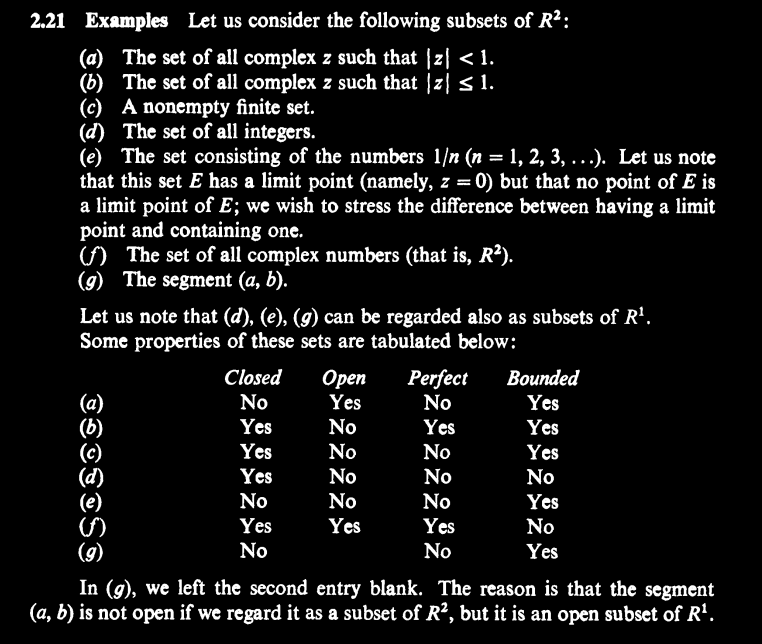
\includegraphics[width=.9\linewidth]{/static/flopen.png}
\end{center}

\textbf{Theorem}

Let \(\left{E_\alpha \right}\) be a collection of sets. Then

\[
\left(\bigcup_\alpha E_\alpha \right)^c = \bigcap_\alpha (E_\alpha^c)
\]


\textbf{Theorem}

A set is open iff its complement is closed

A set F is closed iff its complement is open.

\textbf{Theorem}

\begin{enumerate}
\item For any collection of open sets, \(\{G_\alpha\}\), \(\cup_\alpha G_\alpha\) is open.
\item For any collection of closed sets, \(\{F_\alpha\}\), \(\cap_\alpha G_\alpha\) is closed.
\item For any finite collection of open sets, \(\cap_i G_i\) is open.
\item For any finite collection of closed sets, \(\cup_i F_i\) is closed.
\end{enumerate}


\textbf{Definition}

If X is a metric space, E is a subset of X and if E' is the set of limit points of E in X, then the \textbf{closure} of E is the set \(\bar{E} = E \cup E'\).
in
\textbf{Theorem}

\begin{enumerate}
\item \(\bar{E}\) is closed.
\item \(E = \bar{E}\) iff E is closed.
\item \(\bar{E} \subset F\) for every closed set \(F \subset X\) such that \(E \subset F\).
\end{enumerate}


\textbf{Theorem}
Let E be a nonempty set of real numbers which is bounded above. Let \(y = \sup E\), then \(y \in \bar{E}\). Hence, \(y \in E\) if E is closed.

\textbf{Theorem}

Suppose \(Y \subset X\). A subset E of Y is open relative to Y iff \(E = Y \cap G\) for some open subset G of X.

(???)

\subsection{Compact sets}
\label{sec:org31168bd}

\textbf{Definition}

An \textbf{open cover} of a set E in a metric space X, we mean a collection of open subsets of X such that \(E \subset \cup_\alpha G_\alpha\).

\textbf{Definition}

A subset K of of a metric space X is said to be \textbf{compact} if every open cover of K contains a subcover. i.e. if \(\left\{G_\alpha \right\}\) is an open cover of K, then there are finitely many indices \(\alpha_1, \ldots, \alpha_n\), such that:

\[
K \subset G_{\alpha_1} \cup \ldots \cup G_{\alpha_n}
\]

\textbf{Theorem}

Suppose \(K \subset Y \subset X\). Then K is compact relative to X iff K is compact relative to Y.


\textbf{Theorem}

Compact subsets of metric spaces are closed.

\textbf{Theorem}

Closed subsets of compact sets are compact.
\textbf{Corollary}: If F is closed and K is compact, then \(F \cap K\) is compact.

\textbf{Theorem}

If \(\{K_\alpha\}\) is a collection of compact subsets of a metric space X such that the intersection of every finite subcollection of \(\{\K_alpha\}\) is non-empty, then \(\cap K_\alpha\) is nonempty.
\textbf{Corollary}: If \(\{K_n\}\) is a sequence of nonempty compact sets such that \(K_n \supset K_{n+1}\) then \(\cap_1^\infty K_n\) is not empty.

\textbf{Theorem}
If E is an infinite subset of a compact set K, then E has a limit point in K.

\textbf{Theorem}
If \(\{I_n\}\) is a sequence of intervals in \(R^1\), such that \(I_n \supset I_{n+1}\) then \(\cap^\infty_1 I_n\) is not empty.

\textbf{Theorem}
If \(\{I_n\}\) is sequence of k-cells such that \(I_n \superset I_{n+1}\), then \(\cap^\infty_1 I_n\) is not empty.

\textbf{Theorem}
Every k-cell is compact.

\textbf{Theorem}
If a set in \(R^k\) has one of the following three properties, it has the other two.

\begin{enumerate}
\item E is closed and bounded
\item E is compact
\item Every infinite subset of E has a limit point in E.

(b) and (c) are equivalent in any metric space but (a) does not in general imply (b) and (c).
\end{enumerate}

\textbf{Theorem (Weierstrass)}

Every bounded infinite subset of \(R^k\) has a limit point in \(R^k\).

\subsection{Perfect sets}
\label{sec:org1ecfacd}

\textbf{Theorem}

A nonempty perfect set in \(R^k\) is uncountable.

\subsection{Connected sets}
\label{sec:orgc813c8b}

Two subsets A,B of a metric space X are \emph{seperated} if \(A \cap \bar{B}\) and \(\bar{A}\cap B\) are empty. A subset of X is connected if it is not a union of two nonempty seperated sets.

\textbf{Theorem}

A subset E of the real line \(R^1\) is connected iff it has the following property: If \(x,y \in E\), \(x < z < y\), then \(z \in E\).

\section{Topological spaces}
\label{sec:org0b443d1}

\textbf{Definition}

A topology on a set X is a collection \(\mathcal{T}\) of subsets of X having the following properties.


\begin{enumerate}
\item \(\emptyset\) and X are in \(\mathcal{T}\)
\item The union of the elements of any subcollection of \(\mathcal{T}\) is in \(\mathcal{T}\)
\item The intersection of the elements of any finite subcollection of \(\mathcal{T}\) is in \(\mathcal{T}\)
\end{enumerate}

If X is a topological space with topology \(\mathcal{T}\), we say that a subset U of X is an \textbf{open set} of X if U belongs to the collection \(\mathcal{T}\).


The collection of all subsets of X is called the \textbf{discrete topology}. The collection consisting of X and \(\emptyset\) only is the \textbf{indiscrete/trivial topology}.

Let \(\mathcal{T}_f\) be the collection of all subsets U of X such that X-U either is at most countable or is all of X. Then \(\mathcal{T}_f\) is the \textbf{finite complement topology}.

\textbf{Definition}

Suppose that \(\mathcal{T}\) and \(\mathcal{T}'\) are two topologies. If \(\mathcal{T}' \supset \mathcal{T}\), we say \(\mathcal{T}'\) is \textbf{finer} than \(\mathcal{T}\). If it proper contains \(\mathcal{T}\), we say strictly finer than \(\mathcal{T}\). The reverse is called coarser. \(\mathcal{T}\) is comparable with \(\mathcal{T}'\) if one is the subset of the other.

\subsection{Basis}
\label{sec:orgbd1ee17}

A \textbf{basis} for a topology on X is a collection \(\mathcal{B}\) of subsets of X (called \textbf{basis elements}) such that:

\begin{enumerate}
\item For each \(x \in X\), there is at least one basis element B containing x. (B is a cover)
\item If x belongs to the intersection of two basis elements \(B_1\) and \(B_2\), then there is a basis element \(B_3\) containing x such that  \(B_3 \subset B_1 \cap B_2\).
\end{enumerate}

If \(\mathcal{B}\) satisfies these conditions, we define the topology generated by \(\mathcal{B}\) as: A subset U of X is said to be open in X if for each \(x \in U\), there is a basis element \(B \in \mathcal{B}\) such that \(x \in B\) and \(B \subset U\). Note each element is an element of \(\mathcal{T}\).

\textbf{Lemma}

\(\mathcal{T}\) equals the collection of all unions of elements of \(\mathcal{B}\).

\textbf{Lemma}

Let X be a topological space. Suppose that \(\mathcal{C}\) is a collection of open sets of X such that for each open set U of X and each x in U, there is an element \(C\) of \(\mathcal{C}\) such that \(x \in C \subset U\). Then \(\mathcal{C}\) is a basis for the topology of X. (C make up a cover and open set of X is a superset of some C).

\emph{Proof.} We will show why every element in \(\mathcal{T}\) belongs in the topology generated by the basis, \(\mathcal{T}'\). Since for \(x \in C \subset U\), there exists a union of C which equals U. The converse follows from the previous lemma.


\textbf{Lemma (Fineness)}

Let \(\mathcal{B}\) and \(\mathcal{B}'\) be the bases for topologies \(\mathcal{T}\) and \(\mathcal{T}'\) respectively on X. Then the following are equivalent.

\begin{enumerate}
\item \(\mathcal{T}'\) is finer than \(\mathcal{T}\)
\item For each \(x \in X\), and each basis element \(B \in \mathcal{B}\) containing \(x\), there is a basis element \(B' \in \mathcal{B}'\) s.t. \(x \in B' \subset B\).
\end{enumerate}


\subsubsection{Common topologies}
\label{sec:orgb13d1f5}

\begin{center}
\begin{tabular}{lll}
Topology & Basis & Symbol\\
\hline
Standard & (a,b) & \(\mathbb{R}\)\\
Lower-limit & [a,b] & \(\mathbb{R}_l\)\\
K-topology & (a,b) and (a,b) - K & \(\mathbb{R}_K\)\\
\end{tabular}
\end{center}

Note: K is the set of all numbers \(1/n\) for each positive integer n.

\textbf{Lemma}
Topologies of \(\mathbb{R}_l\) and \(\mathbb{R}_K\) are strictly finer than the standard topology on \(\mathbb{R}\), but are not comparable with one another.

\subsubsection{Subbasis}
\label{sec:org0ea1991}

What if you extend the basis to also take finite intersections?

\textbf{Definition}

A subbasis \(\mathcal{S}\) for a topology on X is a collection of subsets of \(X\) whose union equals X. The topology generated by the subbasis is defined to be the collection \(\mathcal{T}\) of all unions of finite intersections of elements of \(\mathcal{S}\).

\subsection{Order topology}
\label{sec:org3a5faee}

\textbf{Definition}

Let \(X\) be a set with a simple order relation. The collection of all sets of the following types:

\begin{enumerate}
\item All open intervals
\item All intervals of the form \([a_0,b]\) where \(a_0\) is the smallest element if any
\item All intervals of the form \([a,b_0]\) where \(b_0\) is the largest element if any
\end{enumerate}

is the basis for the \textbf{order topology} on X.

\subsection{Product topology}
\label{sec:orga7059a3}

\textbf{Definition}

Let X and Y be topological spaces. The \textbf{product topology} on \(X \times Y\) is the topology having as basis the collection of all sets of the form \(U \times V\), where \(U \in X, V \in Y\).

\textbf{Theorem}

If \(\mathcal{B}\) is the basis for the topology of \(X\) and \(\mathcal{C}\) is a basis topology of Y, then the collection:


\[
\mathcal{D} = \{B \times C \vert B \in \mathcal{B}, C \in \mathcal{C}\}
\]

is a basis for the topology of \(X \times Y\).


We are also interested in a subbasis.

\textbf{Theorem}

\[
\mathcal{S} = \{\pi_1^{-1}(U) \vert U \text{ open in } X \} \cup \{\pi_2^{-1}(V) \vert V \text{ open in } Y \}
\]

\subsection{Subspace topology}
\label{sec:orge8897f5}

\textbf{Definition}

Let X be a topological space with topology \(\mathcal{T}\). If \(Y \subset X\),

\[
\mathcal{T}_Y = \{Y \cap U \vert U \in \mathcal{T}\}
\]

is the \textbf{subspace topology} on \(Y\). Y is then a \textbf{subspace} of X,

\textbf{Lemma}

A basis can be derived in a similar form. (replace Y with B).

\textbf{Lemma}

If \(U\) is open in \(Y\) and \(Y\) is open in \(X\), then \(U\) is open in \(X\).

\textbf{Definition}

A subset Y of X is convex in X if for each pair of points \(a < b\) of Y, the entire interval of points of X lies in Y.


\textbf{Theorem}

Let \(X\) be an ordered set in the order topology, let Y be a subset of X that is convex in X. Then the order topology on Y, is the same as the topology Y inherits as a subspace of X.


\subsection{Closed sets}
\label{sec:org382a78b}

Defining topological space with closed sets.

\textbf{Theorem}

In a topological space,

\begin{enumerate}
\item the empty set and the whole set are closed
\item Arbitrary intersections of closed sets are closed
\item Finite unions of closed sets are closed
\end{enumerate}

\subsubsection{Closures}
\label{sec:org60f728e}

\textbf{Theorem}

Let A be a subset of the topological space X.
\begin{enumerate}
\item Then \(x \in \bar{A}\) iff every neighbourhood of x intersects A.
\item If X is given by a basis, \(x \in \bar{A}\) iff every basis element containing x intersects A.
\end{enumerate}

\subsection{Hausdorff spaces}
\label{sec:org8681341}

Usually it is nicer to have one-point sets closed like in euclidean space, as this means that sequences don't converge to multiple values for instance.

\textbf{Definition}

A topological space X is a \textbf{Hausdorff space}, if for each pair of distinct points in X, there exist neighborhoods of each point that are disjoint.

\textbf{Theorem}

Every finite point set in a hausdorff space is closed.

The Hausdorff space condition is stronger than the condition that finite point sets be closed (\(T_1\) axiom) but that's fine. But for fun:

\textbf{Theorem}

Let X be a space satisfying the \(T_1\) axiom. Let A be a subset of X, then the point x is a limit point of A iff every neighbourhood of x contains infinitely many points of A.

Back to hausdorff spaces:

\textbf{Theorem}

Every simply ordered set is a Hausdorff space in the order topology. Product and subspaces of hausdorff spaces are hausdorff spaces.
\subsection{Continuous functions}
\label{sec:orgd127057}

\textbf{Definition}

A function \(f : X \to Y\) is continuous if for each open subset V of Y, the set \(f^{-1}(V)\) is an open subset of X.

It also suffices to show that the inverse image of each basis/subbasis element is open.

Other definitions:

\textbf{Theorem}

\begin{enumerate}
\item For every subset of X, one has \(f(\bar{A}) \subset \bar{f}(A)\).
\item For every closed set of B of Y, the set \(f^{-1}(B)\) is closed in X.
\item For every \(x \in X\) and each neighbourhood \(V\) of f(x), there is a neighbourhood \(U\) of x such that \(f(U) \subset V\).
\end{enumerate}

\textbf{Definition}

If \(f\) is an injective continuous map, and f' is the surjective function by restricting the range of f, f is a topological imbedding if f' is a homeomorphism of X with Z.



\subsubsection{Homeomorphisms}
\label{sec:orgd80a8d2}

Let \(f : X \to Y\) be a bijection. If both \(f\) and its inverse function are continuous, \(f\) is called a homeomorphism.
Another way to define it is to say it is a bijective correspondence such that \(f(U)\) is open iff U is open.

\subsection{Metric topology}
\label{sec:org07aab22}

\textbf{Definition}

The collection of all \$\(\epsilon\)\$-balls \(B_d(x,\epsilon)\) is a basis for a topology on X, called the \textbf{metric topology}, induced by d.

\textbf{Definition (alt)}

A set U is open in the metric topology induced by d iff for each \(y \in U\), there is a \(\delta > 0\) s.t. \(B_d(y,\delta) \subset U\).

\textbf{Definition}

A topological space X is \textbf{metrizable} if there exists a metric on X that induces the topology of X. A \textbf{metric space} is a metrizable space together with a specific metric that gives the topology of X.

\textbf{Lemma (Sequence lemma)}

Let \(X\) be a topological space. Let \(A \subset X\). If there is sequence of points of \(A\) converging to \(x\), then \(x \in \bar{A}\). the converse holds if \(X\) is metrizable.


\textbf{Theorem}

Let \(f : X \to Y\). If the fucntion if is continuous, then for every convergent sequence \(x_n \to x\) in X, the sequence \(f(x_n)\) converges to \(f(x)\). The converse holds if \(X\) is metrizable.

\textbf{Theorem (Uniform limit theorem)}

Let \(f_n : X \to Y\) be a sequence of continuous functions from the topological space \(X\) to the metric space \(Y\). If \((f_n)\) converges uniformly to \(f\), then \(f\) is continuous.

\subsection{Quotient topology}
\label{sec:orga386c8b}

\textbf{Definition}

Let X and Y be topological spaces; let \(p : X \to Y\) be a surjective map. The map \(p\) is said to be a quotient map provided a subset \(U\) of \(Y\) is open in Y if and only if \(p^{-1}(U)\) is open in X.

(like a homeomorphism without being injective)


\textbf{Definition}

A subset \(C\) of \(X\) is saturated (with respect to the surjective map) if \(C\) contains every set \(p^{-1}({y})\) it intersects. Thus \(C\) is saturated if it equals the complete inverse image of a subset of \(Y\). To say that \(P\) is a quotient map is equivalent to saying that \(p\) is continuous and \(p\) maps saturated open sets of \(X\) of to open sets of \(Y\).

A map is an open set if for each open set in its domain, its image is also open, and likewise for closed maps. All open/closed maps are quotient maps.

\textbf{Definition}

If X is a space and A is a set and if \(p:X\to A\) is a surjective map, there is exactly one topology \(\mathcal{T}\) on A relative to which p is a quotient map, which is the \textbf{quotient topology} induced by p.

\textbf{Definition}

Let \(X\) be a topological space, and let \(X^*\) be a partition of \(X\) into disjoint subsets whose union is \(X\). Let \(p : X \to X^*\) be the surjective map that carries each point of \(X\) to the element of \(X^*\) containing it. In the quotient topology induced by \(p\), the space \(X^*\) is called a \textbf{quotient space} of X.

What concepts do quotient maps work well with?

\subsubsection{Subspaces}
\label{sec:org3ac9669}

\textbf{Theorem}

Let \(p : X \to Y\) be a quotient map; let A be a subspace of X that is saturated with respect to p.; let \(q: A \to p(A)\) be the map obtained by restricting p.

\begin{enumerate}
\item If A is either open or closed in X, then q is a quotient map
\item If p is either an open map or a closed map, then q is a quotient map.
\end{enumerate}


\subsubsection{Composites}
\label{sec:org9fa573a}

Composites of quotient maps are quotient maps.

\subsubsection{Products}
\label{sec:org2a6e449}

Products of maps do not behave well, and one needs conditions such as local compactness, and that the two maps are open maps.

\subsubsection{Hausdorff condition}
\label{sec:org9071500}

Does not behave well.

For \(X^*\) to satisfy the \(T_1\) axiom, one requires that each eleemtn of the partition \(X^*\) be a closed subset of \(X\).


\subsubsection{Continuous functions}
\label{sec:orge599d90}

Similar to how we had a criterion for determining when a map into a product space was continuous, we wish to find when a map out of a quotient space is continuous.

\textbf{Theorem}

Let \(p:X\to Y\) be a quotient map. Let \(Z\) be a space and let \(g : X \to Z\) be a map that is constant on each set \(p^{-1}({y})\) for \(y \in Y\). Then \(g\) induces a map \(f : Y \to Z\) such that \(f \circ p = g\). The induced map \(f\) is continuous iff g is continuous; f is a quotient map iff g is a quotient map.

\textbf{Corollary}

Let \(g : X \to Z\) be a surjective continuous map. Let \(X*\) be the following collection of subsets of \(X\):

\[
X^* = \{g^{-1}(\{z\}) \vert z \in Z\}
\]

Give it the quotient topology.

\begin{enumerate}
\item The map g induces a bijective continuous map f, which is a homeomorphism iff g is a quotient map
\item If \(Z\) is Hausdorff, so is \(X^*\).kk
\end{enumerate}


\subsubsection{Topological Groups}
\label{sec:org27ae829}

A \textbf{topological group} G is a geoup that is also a topological space satisfying the \(T_1\) axiom, such that the map of \(G \times G\) into \(G\) sending \(x x y\) into \(x \dot y\) and the map of G into G sending x into 1/x are continuous maps.

\section{Connectedness and compactness}
\label{sec:orge7740ff}

\subsection{Connected spaces}
\label{sec:orgaa1aeca}

\textbf{Definition}

Let \(X\) be a topological space. A \textbf{seperation} of X is a pair of disjoint nonempty open subsets of X whose union is X. The space is \textbf{connected} if there does not exist a seperation of X.

Note that connectedness is a topological property.

Another formulation of connectedness is that a space is connected iff the only subsets that are both open and closed in X are the empty set and X itself.

For a subspace of a topological space, there is another useful formulation.

\textbf{Lemma}

If Y is a subspace of X, a seperation of Y is a pair of disjoint nonempty sets A and B whose union is Y. neither of which contains a limit point of the other. The space Y is connected if there exists no seperation of Y.

\subsubsection{Forming connected spaces from given ones}
\label{sec:org7c36aa5}

\textbf{Lemma}

If the sets C and D form a seperation of X, and if Y is a connected subspace of X, then Y lies entirely within either C or D.

\textbf{Properties:}
\begin{enumerate}
\item The union of a collection of connected subspaces of X that have a point in common is connected.
\item Let A be a connected subspace of X. If \(A \subset B \subset \bar{A}\), then B is also connected.
\item The image of a connected space under a continuous map is connected.
\item A finite cartesian product of connected spaces is connected.
\end{enumerate}


\subsection{Connected subspaces of the real line}
\label{sec:orgc19ee85}

A simply ordered set L having more than one element is called a \textbf{linear continuum} if the following hold:

\begin{enumerate}
\item L has the least upper bound property
\item If \(x < y\), there exists \(z\) such that \(x < z < y\)
\end{enumerate}

\textbf{Theorem}

If L is a linear continuum in the order topology, then L is connected, and so are intervals and rays in L.

\textbf{Corollary}

The real line is connected and so are intervals and rays

\textbf{Theorem (Intermediate value theorem)}

Let \(f : X \to Y\) be a continuous map, where X is a connected space and Y is an ordered set in the order topology. If a and b are two points of X and if r is a point of Y lying between f(a) and f(b), then there exists a point c of X such that f(c) = r.

\subsection{Path connectedness}
\label{sec:org31a079d}

\textbf{Definition}

Given points x and y of the space X, a \textbf{path} in X from x to y is a continuous map \(f : [a,b] \to X\) of some closed interval in the real line into X, such that f(a) = x and f(b) = y. A space X is said to be path connected if every pair of points of X can be joined by a path in X.


Although a path-connected space is connected, the converse may not hold (Such as the ordered square).

\subsection{Components and local connectedness}
\label{sec:org9c6c117}

\textbf{Definition}

Given X, define an equivalence relation on X by setting \(x \tilde y\) if there is a connected subspace of X containing both x and y. The equivalence classes are the components of X.

\textbf{Theorem}

The components of X are connected disjoint subspaces of X whose union is X. such that nonempty connected subspace of X intersects only one of them.

\textbf{Theorem}

the path components are defined similarly, with an equivalence relation when there is a path from x to y in X.

\textbf{Theorem}

The path components of X are path-connected disjoint subpaces of X whose union is X, such that each nonempty path-connected subspace of X intersects only one of them.


\textbf{Definition}

A space X is said to be \textbf{locally connected at x}, if for every neighbourhood U of x, there is a connected neighborhood V of x contained in U. If X is locally connected at each of its points, it is said simply to be locally connected. Similarly, a space is \textbf{locally path connected at x} if for every neighbourhood U of X, there is a path-connected neighborhood V of x contained in U.

\textbf{Theorem}

A space X is locally connected iff for every open set U of X, each component of U is open in X.

\textbf{Theorem}

A space X is locally path connected iff for every open set U of X, each path component of U is open in X.

\textbf{Theorem}

If X is a topological space, each path component of X lies in a component of X. If X is locally path connected, then the components and the path components of X are the same.


\subsection{Compact spaces}
\label{sec:org62b9296}

\textbf{Definition}

A space X is \textbf{compact} if every open covering A of X contains a finite subcollection that also covers X.

\textbf{Theorem}

Every closed subspace of a compact space is compact.

\textbf{Theorem}

Every compact subspace of a Hausdorff space is closed

\textbf{Lemma}

If Y is a compact subspace of the Hausdorff space X and \(x_0\) is not in Y, then there exist disjoint open sets U and V of X containing \(x_0\) and Y, respectively.

\textbf{Theorem}

The image of a compact space under a continuous map is compact.


\textbf{Theorem}

Let \(f : X \to Y\) is a bijective continuous function. If X is a compact and Y is Hausdorff, then f is a homeomorphism

Useful for proving a map is a homeomorphism.

\textbf{Theorem}

The product of finitely many compact spaces is compact.

\textbf{Lemma (The tube lemma)}

Consider the product space \(X \times Y\), where Y is compact. If N is an open set of \(X \times Y\) containing the slice \(x_0 \times Y\) of \(X \times Y\), then N contains some tube \(W \times Y\) about \(x_0 \times Y\), where \(W\) is a neighbourhood of \(x_0\) in X.


For infinite products, we require the Tychanoff theorem.


\subsubsection{Finite intersection}
\label{sec:org835b3c7}

Following is another formulation of compactness.

\textbf{Definition}

A collection \(\mathcal{C}\) of subsets of X is said to have the \textbf{finite intersection property} if for every finite subcollection, its intersection is nonempty.

\textbf{Theorem}

Let X be a topological space. Then X is compact iff for every collection of closed sets in X having the finite intersection property, the intersection of all its elements is nonempty.

\subsection{Compact subspaces of the real line}
\label{sec:org461f6ce}

\textbf{Theorem}


Let X be a simply ordered set having the least upper bound property. In the order topology, each closed interval in X is compact.

\textbf{Corollary}

Every closed interval in \(\mathbb{R}\) is compact

\textbf{Theorem}

A subspace A of \(R^n\) is compact iff it is closed and bounded in the euclidean or square metric.


\textbf{Theorem (EVT)}

Let \(f : X \to Y\) be continuous, where Y is an ordered set in the order topology. If X is compact, then there exist points c and d in X such that \(f(c) \leq f(x) \leq f(d)\) for every \(x \in X\).

\subsubsection{Uniform continuity theorem}
\label{sec:org0bd582b}

\textbf{Definition}

Let (X,d) be a metric space. let A be a nonempty subst of X. For each \(x \in X\), we define the distance from x to A by the equation:

\[
d(x,A) = \inf \{d(x,a) \vert a \in A\}
\]

\textbf{Lemma (The Lebesgue number lemma)}

Let \(\mathcal{A}\) be an open covering of the metric space (X,d). If X is compact, there is a \(\delta > 0\) such that for each subset of X having diameter less that \(\delta\), there exists an element of \(\mathcal{A}\) containing it.

\(\delta\) is known as the \textbf{Lebesgue number}.

\textbf{Definition}

A function f fomr the metric space \((X,d_X)\) to the metric space \((Y,d_Y)\) is said to be \textbf{uniformly continuous} if given \(\epsilon > 0\), there is a \(\delta > 0\) such that for every pair of points \(x_0,x_1\) of X.

\textbf{Theorem (Uniform continuity theorem)}

Let \(f : X \to Y\) be a continuous map of the compact metric space (X,dx) to the metric space (Y,dy). Then f is uniformly continuous.


\subsubsection{Uncountability of real numbers}
\label{sec:org98b9eff}

\textbf{Definition}

A point x of a space X is said to be an \textbf{isolated point} of X if the one-point set \(\{x\}\) is open in X.

\textbf{Theorem}

Let X be a nonempty compact Hausdorff space. If X has no isolated points, then X is uncountable.

\textbf{Corollary}

Every closed interval in \(\mathbb{R}\) is uncountable.



\subsection{Limit point compactness}
\label{sec:org8e979fc}

Also known as \textbf{Frechet compactness}, or \textbf{Bolzano-Weierstrass property}, and was the former definition of compactness whereas the covering formulation was called "bicompactness".

\textbf{Theorem}

Compactness implies limit point compactness, but not conversely.

\textbf{Definition}

Let X be a topological space. It is \textbf{sequentially compact} if every sequence of points of X has a convergent subsequence.

But metrizable spaces are very nice so:

\textbf{Theorem}

Let \(X\) be a metrizable space. Then the three defintions of compactness are equivalent.


\subsection{Local compactness}
\label{sec:org7ee03dc}

We wish to prove the basic theorem that any locally compact Hausdorff space can be imbedded in a certain compact Hausdorff space that is called its \textbf{one-point compactification.}

\textbf{Definition}

A space X is said to be \textbf{locally compact at x} if there is some compact subspace C of X that contains a neighbourhood of x.

Metrizable spaces and compact Hausdorff spaces are very well behaved. A subspace of a metrizable space is also metrizable but the subspace of a compact Hausdorff space need not be compact.

\textbf{Theorem}

Let X be a space. Then X is locally compact hausdorff iff there exists a space Y satisfying the following conditions:

\begin{enumerate}
\item X is a subspace of Y.
\item The set Y - X consists of a single point.
\item Y is a compact Hausdorff space.
\end{enumerate}

If there are two spaces satisfying these conditions, then there is a homeomorphism between them that equals the identity map on X.

\textbf{Definition}

If Y is a compact Hausdorff space and X is a proper subspace of Y whose closure equals Y, then Y is said to be a \textbf{compactification} of X. If Y-X equals a single point, then Y is called the \textbf{one-point compactification} of X.


But our definition of local compactness does not involve arbitrarily small neighbourhoods like the other definitions. Thus, here is a definition which is equivalent when X is Hausdorff.

\textbf{Theorem}

Let X be a Hausdorff space. Then X is locally compact iff given x in X, and given a neighborhood U of x, there is a neighbourhood V of x such that \(\bar{V}\) is compact and \(\bar{V}\subset U\).

\textbf{Corollary}

Let X be locally compact Hausdorff; Let A be a subspace of X. If A is closed/open in X, then A is locally compact.

If A is closed, we don't need the Hausdorff condition.

\textbf{Corollary}

A space X is homeomorphic to an open subspace of a compact Hausdorff space iff X is locally compact Hausdorff.

This follows from the previous corollary and the second last theorem.

\section{Countability and Seperation axioms}
\label{sec:org793c388}

We wish to prove the Urysohn metrization theorem, which says that if a topological space satisfies a certain countability axiom (the second) and a certain seperation axiom (the regularity axiom), then X can be imbedded in a metric space and is thus metrizable.

Another imbedding theorem useful in geometry is that given a space that is a compact manifold, we show that it can be imbedded in some finite dimensional euclidean space.

\subsection{Countability Axioms}
\label{sec:org78b3aa7}

\textbf{Definition}

A space X is said to have a \textbf{countable basis at x} if there is a countable collection \(\mathcal{B}\) of neighbourhoods of x such that each neighbourhood of x contains at least one of the elements of \(\mathcal{B}\). A space that has a countable basis at each of its points is said to satisfy the \textbf{first countability axiom}, or be \textbf{first-countable}.

\textbf{Theorem}

Let X be a topological space.

\begin{enumerate}
\item Let A be a subset of X. If there is a sequence of points A converging to x, then \(x\in \bar{A}\). The converse holds if X is first-countable.
\item Let \(f: X \to Y\). If f is continuous, then for every convergent sequence \(x_n \to x\) in X, the sequence \(\{x_n\}\) converges to \(f(x)\). The converse holds if X is first-countable.
\end{enumerate}

\textbf{Definition}

If a space X has a countable basis for its topology, then X is said to satisfy the \textbf{second countability axiom}, or to be \textbf{second-countable}.


This axiom implies the first, and is usually satisfied by familiar spaces.

\textbf{Theorem}

A subspace of a first-countable space is first-countable, and a countable product of first-countable spaces if first-countable. A subspace of a second-countable space is second-countable, and a countable product of second-countable spaces is second-countable.

\textbf{Definition}

A subset A of X is said to be \textbf{dense} in X if \(\bar{A} = X\).

\textbf{Theorem}

Suppose X has a countable basis. Then:
\begin{enumerate}
\item Every open covering of X contains a countable subcollection covering X. (\textbf{Lindelof space})
\item There exists a countable subset of X that is dense in X. (\textbf{seperable})
\end{enumerate}


\subsection{Seperation axioms}
\label{sec:org49d98d2}

We will introduce seperation axioms stronger than Hausdorff.

\textbf{Definition}

Suppose that one-point sets are closed in X. Then X is said to be \textbf{regular} if for each pair consisting of a point x and a closed set B disjoint from X, there exist disjoint open sets containing x and B, respectively. The space X is said to be \textbf{normal} if for each pair A,B of disjoint closed sets of X, there exist disjoint open sets containing A and B, respectively.

A regualar space is Hausdorff and a normal space is regular (Though we need to include the condition that one-point sets be closed. See the two-point space in the indiscrete topology satisfies the other parts of the definitions of regularity and normality without being Hausdorff).

\textbf{Lemma}

Let X be a topological space. Let one-point sets in X be closed.

\begin{enumerate}
\item X is regular iff given a point x of X and a neighbourhood U of x, there is a neighbourhood V of x such that \(\bar{V}\subset U\).
\item X is normal iff given a closed se A and an open set U containing A, there is an open set V containing A such that \(\bar{V} \subset U\).
\end{enumerate}


\textbf{Theorem}

\begin{enumerate}
\item A subspace of a Hausdorff space is Hausdorff; a product of Hausdorff spaces is Hausdorff.
\item A subspace of a regular space is regular; a product of regular spaces is regular
\end{enumerate}

But there is no analagous theorem for normal spaces
\end{document}